\documentclass[a4paper]{ltjsarticle}
\usepackage{color}
\usepackage{comment}
\usepackage[bottom=25mm]{geometry} % 余白等の設定
\usepackage{lastpage} % 最後のページ番号を \pageref{LastPage} で取得
\usepackage{fancyhdr} % ヘッダー
\usepackage{titlesec} % Section などの設定
\usepackage[unicode]{hyperref} % PDF のメタデータ生成
\usepackage{docmute}

\usepackage{amsfonts} % 整数全体の集合とかの記号を表すフォント
\usepackage{bm}       % 数式でベクトルを表す太字斜体
\usepackage{braket}   % Dirac の Braket 記法

\usepackage[version=4]{mhchem}   % 化学式
\usepackage{chemfig}  % 構造式
\usepackage{siunitx}  % SI unit
\usepackage{listing}  % コード

\makeatletter

% maketitle
\@addtoreset{section}{part}
\titleformat{\part}{\centering\Large}{}{0em}{}
\titlespacing{\part}{0pt}{0ex}{1cm}
\newcommand{\repotitle}[1]{\def\@repotitle{#1}}
\newcommand{\gakuseinumber}[1]{\def\@gakuseinumber{#1}}
\renewcommand{\maketitle}{
    % 表紙にするときはコメントアウト
    \thispagestyle{empty}
    \pagenumbering{gobble}
    \vspace*{\stretch{1}}
    \begin{center}
        \vspace*{0.4cm}
        {\Huge{\@title}}
        \vspace{1cm}

        {\Large \@date}

        \vspace{0.5cm}

        {\Large \@gakuseinumber \quad \@author}

        \vspace{1cm}
    \end{center}
    \vspace{\stretch{1}}
    \newpage
    \pagenumbering{arabic}
}


% Header
\pagestyle{fancy}
\lhead{\@repotitle \qquad \@gakuseinumber \quad \@author}
\rhead{Page \thepage\ of \pageref{LastPage}}
\fancyfoot{}
\fancypagestyle{nofooter}
\makeatother

% Macros
\newcommand{\uL}[0]{\si{\micro L}}
\newcommand{\ug}[0]{\si{\micro g}}

%%%% Title %%%%%%%%%%%%%%%%%%%%%%%%%%%%%%%%%%%%%%%%%%%%%%%%%%%%%%%%%%%%%%%%%%%%%
\repotitle{分析化学実験 5 レポート}
\title{分析化学実験 5 レポート \\ \vspace{1.5ex} {\LARGE --- 生化学分析 ---}}
\author{宗形 翼}
\gakuseinumber{03-200796}
\date{\today}
\hypersetup{
    pdftitle={分析化学実験 5 レポート},
    pdfauthor={宗形 翼}
}

\begin{document}

\part{実験A 免疫分析}

% ____
% |  _ \ _   _ _ __ _ __   ___  ___  ___
% | |_) | | | | '__| '_ \ / _ \/ __|/ _ \
% |  __/| |_| | |  | |_) | (_) \__ \  __/
% |_|    \__,_|_|  | .__/ \___/|___/\___|
%                  |_|
\section{目的}

サンドイッチ法のERISAにより、代表的な抗原であるヒトIgGを定量する。
ERISA に特有な High-dose hook effect を経験し、
B/F分離の有効性と欠点について考察する。

%  _____                      _                      _
% | ____|_  ___ __   ___ _ __(_)_ __ ___   ___ _ __ | |_
% |  _| \ \/ / '_ \ / _ \ '__| | '_ ` _ \ / _ \ '_ \| __|
% | |___ >  <| |_) |  __/ |  | | | | | | |  __/ | | | |_
% |_____/_/\_\ .__/ \___|_|  |_|_| |_| |_|\___|_| |_|\__|
%            |_|
\section{実験}


\subsection{器具}

\begin{itemize}
    \item マイクロタイター用比色計
    \item 恒温槽(37℃)
    \item 冷蔵庫(5℃)
    \item 攪拌器
    \item ELISA用マイクロタープレート
    \item 連続分注ピペット
    \item マイクロピペット
    \item 試験管
    \item 試験管立て
\end{itemize}

\subsection{試薬}

\begin{itemize}
    \setlength\parskip{1em}
    \item 0.1 M 炭酸緩衝液 \\
    炭酸ナトリウム 2.52 g と炭酸水素ナトリウム 8.4 g を水 1 L に混合する。

    \item 1/15 Mリン酸緩衝液 (PBS) \\
    リン酸二水素カリウム2.73 gとリン酸水素二ナトリウム・12水和物
    16.8 gを水 1 Lに溶解し、塩化ナトリウムを最終濃度が0.08\% になるように加える。この溶液
    の pH は7.2である。

    \item 1/15 M リン酸--Tween20 緩衝液 (PBS-T) \\
    PBS 溶液に濃度が 0.05\%となるように界面活性剤 Tween20 を加える。

    \item リン酸緩衝液--牛血清アルブミン溶液 (PBS-B) \\
    リン酸緩衝液(PBS)に
    牛血清アルブミンを最終濃度 1\%になるように加え、泡がたたないように徐々に溶解する。

    \item リン緩衝液--Tween20 牛血清アルブミン溶液(PBS-TB) \\
    PBS-T 溶液に牛血清アルブミン
    を最終濃度 \%になるように加え、泡がたたないように徐々に溶解する。

    \item クエン酸--リン酸緩衝液 \\
    水 1 L にクエン酸一水和物 5.1 g およびリン酸水素二ナトリウム
    12水和物 18.4 g を溶かす(pH 5.0)。

    \item 抗ヒト IgG 溶液 (20 \si{\micro g/mL}) \\
    試験管に抗ヒト IgG 原液 (2.4 mg /mL)をマイクロピペットで
    33.34 \uL 計りとり、これに 0.1 M 炭酸緩衝液 4 mL を加えて良くふりまぜる。

    \item ヒト IgG 溶液 (16.0 \ug/mL) \\
    ヒト IgG 2.76 \uL をガラス試験管にはかりとり、PBS-T 溶液 2 mL を加えて良く混ぜる。

    \item 抗ヒト IgG-ペルオキシダーゼ(HRP)溶液 \\
    原液 0.5 \uL に PBS-TB 溶液 4 mL を加える(8000倍に希釈)

    \item 基質溶液 \\
    o-フェニレンジアミン 60 mg を 100 mL ビーカーにはかりとり、
    これにクエン酸--リン酸緩衝液 20mL を加え、スターラーを使用して溶解する。
    使用直前に 5 \% 過酸化水素水 100 \uL を加えてよく混ぜる。

    \item 5\% 過酸化水素水
    \item 2 M 硫酸
\end{itemize}

\subsection{操作}

\subsubsection{抗体感作}

抗ヒトIgGをELISAプレートに吸着させる。
抗ヒト IgG (20 \ug / mL) 溶液を2個のELISAプレートに
連続分注ピペットを用いて 100 \uL ずつ各穴に分注し、
37℃恒温槽中に1時間放置する。
以後2つのプレートに同じ操作をする。

ELISAプレートを裏返して勢いよく溶液を除去し、
紙で表面の溶液を吸い取る。
これに PBS 溶液を 200 \uL ずつ全ての穴に連続分注ピペットで
分注浸透する。この操作(プレート洗浄操作)を三回繰り返す。

ELISAプレートを裏返して勢いよくPBS溶液を除去し、紙で表面の溶液を吸い取る。
これに PBS-B 溶液を 200 \uL ずつ全ての穴に連続分注ピペットで
分注し、ラップをかぶせ 37℃ 恒温槽中に1時間放置する。

プレート洗浄操作を三回繰り返す。

\subsubsection{抗原抗体反応}

ヒトIgG (16 \ug / mL) 溶液を14本の試験管に
PBS-T 溶液を用いて倍数希釈を行い、
各 1 mL に調整する。
この溶液をマイクロピペットも用いて、ELISAプレートに
希薄溶液から順に 100 \uL ずつ分注する。
このほかに対照として PBS-T 溶液のみを一点とる。
これにラップをかぶせ、37°の恒温槽中に20分間以上放置する。

\subsubsection{酵素標識抗体の抗原抗体反応}

ここまで用意した2個のELISAプレートの内一つに対して、
ヒトIgG溶液に抗ヒト IgG-HRP 溶液 100 \uL
ずつを全ての穴に連続分注ピペットで分注し、
ラップをかぶせ37℃の恒温槽中で20分間放置し、
ELISAプレートをPBS-T 溶液で2回、PBS溶液で1回洗浄する。

もう一つのELISAプレートには、
PBS-T 溶液で2回、PBS溶液で1回洗浄した後に
先ほどのプレート同様な操作を行う。

\subsubsection{基質の酵素反応と定量操作}

調製直後の基質溶液を 100 \uL ずつELISAプレートの全ての穴に
連続分注ピペットで分注する。
30秒程度室温に放置し、着色を確認後
2M 硫酸 25 \uL ずつを全てのあなに連続分注ピペットを用いて加え、
酵素反応を停止させる。

マイクロプレートリーダを用い、波長 490 nm で各穴の吸光度を測定する。


%  ____                 _ _
% |  _ \ ___  ___ _   _| | |_
% | |_) / _ \/ __| | | | | __|
% |  _ <  __/\__ \ |_| | | |_
% |_| \_\___||___/\__,_|_|\__|
%
\section{結果}

ヒトIgG濃度と吸光度を片対数グラフにプロットし図 \ref{fig:a-kenryo} に示した。
洗浄ありのデータから以下のシグモイド曲線に最小二乗法でフィッティングし、
検量線を作成し図中に書き加えた。

$$ f(x) = \frac{a}{1 + \exp(-bx - c)} + d $$

洗浄を行ったものは 1 \ug / mL 程度以上のものは吸光度が飽和した。
一方洗浄を行わなかったものは 0.2 \ug / mL 以上から High-dose hook effect が現れ、
分析値を過小評価してしまう危険性がわかった。


\begin{figure}[htbp]
    \begin{center}
        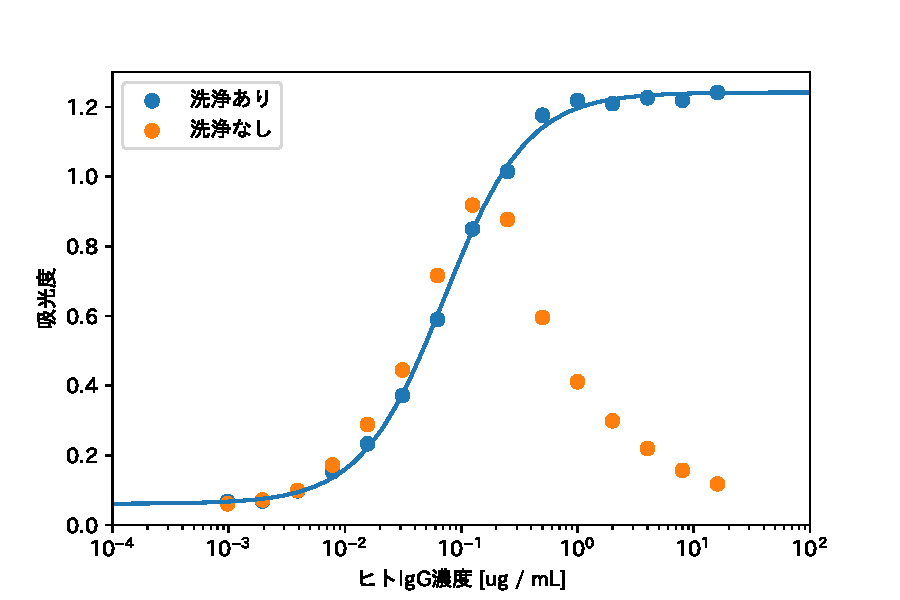
\includegraphics[width=0.8\textwidth]{A-kenryo.pdf}
        \caption{2次多項式近似による検量線}
        \label{fig:a-kenryo}
    \end{center}
\end{figure}

%  ____  _                        _
% |  _ \(_)___  ___ _   _ ___ ___(_) ___  _ __
% | | | | / __|/ __| | | / __/ __| |/ _ \| '_ \
% | |_| | \__ \ (__| |_| \__ \__ \ | (_) | | | |
% |____/|_|___/\___|\__,_|___/___/_|\___/|_| |_|
%
\section{考察}

設問(5)の操作を行ったことによって、
過抗原領域で過小評価を避けることができるようになった。

%  ____            _     _
% |  _ \ _ __ ___ | |__ | | ___ _ __ ___
% | |_) | '__/ _ \| '_ \| |/ _ \ '_ ` _ \
% |  __/| | | (_) | |_) | |  __/ | | | | |
% |_|   |_|  \___/|_.__/|_|\___|_| |_| |_|
%
\section{設問}

\subsection{(1)}

2, 4, 6, 7 の操作について、溶液を丁寧に除去することで過小評価を防ぐ。

6 の操作について、他の穴に溶液が混入しないように注意する。

8 の操作について、硫酸を気質を加えた順番と同じ順序で入れることで、
反応時間が等しくなるようにする。


\subsection{(2)}

操作2はELISAプレートに固定した抗ヒトIgGにヒトIgGを結合させる操作である。

操作3は操作2で結合した抗原に酵素で評した抗体を結合させるための操作である。

\subsection{(3)}

ホモジニアス法は操作が簡単だが High-dose hook effect が起こりやすい。

\subsection{(4)}

低濃度領域では吸光度を測定するときのバックグラウンドの影響が大きくなるから。

また高濃度領域では、ELISAプレートに固定した抗体の
ほとんど全てに抗原が結合することになり、
標的認識抗体と結合しない抗原が多くなるから。

\subsection{(5)}

遊離している抗原を減らせば良いので、PBS 溶液で洗浄する。

%  _____ _
% |  ___(_) __ _ _   _ _ __ ___  ___
% | |_  | |/ _` | | | | '__/ _ \/ __|
% |  _| | | (_| | |_| | | |  __/\__ \
% |_|   |_|\__, |\__,_|_|  \___||___/
%          |___/

\end{document}
